\documentclass[aspectratio=169, xcolor=dvipsnames]{beamer}

% Packages
\usepackage[utf8]{inputenc}
\usepackage{graphicx}
\usepackage{colortbl} % rowcolor support for tables
\usepackage{tabularx} % flexible tables
\usepackage{tikz}
\usepackage{amsmath}
\usetikzlibrary{fadings}
\usepackage{amssymb}
\usepackage{xcolor}
\usepackage{hyperref}
\usepackage{fontawesome5}
\usepackage{multicol}
\usetikzlibrary{positioning, fit, arrows.meta} % For TikZ positioning
\usepackage{tabularx} % For tabular environment in nodes
\usepackage{listings}
\usetikzlibrary{calc}

% TikZ Libraries
\usetikzlibrary{shapes, arrows, positioning, fit, shadows, calc}

% Custom Colors
\definecolor{Primary}{RGB}{255, 152, 0}       % Orange
\definecolor{Secondary}{RGB}{41, 88, 255}     % Blue
\definecolor{Accent}{RGB}{76, 175, 80}        % Green
\definecolor{DarkBg}{RGB}{30, 30, 30}         % Dark Background
\definecolor{LightBg}{RGB}{240, 240, 240}     % Light Background
\definecolor{Warning}{RGB}{255, 87, 34}       % Red-Orange

% Theme Customization
\usetheme{Madrid}
\usecolortheme{default}

% Custom Color Scheme
\setbeamercolor{structure}{fg=Primary}
\setbeamercolor{alerted text}{fg=Warning}
\setbeamercolor{block title}{bg=Primary, fg=white}
\setbeamercolor{block body}{bg=Primary!10, fg=black}
\setbeamercolor{title}{fg=Primary}
\setbeamercolor{subtitle}{fg=Secondary}
\setbeamercolor{frametitle}{bg=Primary, fg=white}
\setbeamercolor{section in toc}{fg=Primary}

% Custom Footer
\setbeamertemplate{footline}{
    \hbox{%
        \begin{beamercolorbox}[wd=0.5\paperwidth,ht=2.25ex,dp=1ex,left]{title in head/foot}%
            \usebeamerfont{title in head/foot}\hspace*{2ex}\insertshortauthor
        \end{beamercolorbox}%
        \begin{beamercolorbox}[wd=0.5\paperwidth,ht=2.25ex,dp=1ex,right]{date in head/foot}%
            \usebeamerfont{date in head/foot}\insertframenumber{} / \inserttotalframenumber\hspace*{2ex}
        \end{beamercolorbox}}%
    \vskip0pt%
}

% Title Page Style
\setbeamertemplate{title page}{
    \begin{tikzpicture}[remember picture, overlay]
        % Background image
        \node[anchor=center] at (current page.center) {
            \IfFileExists{imagebackground.png}{%
                \includegraphics[width=\paperwidth,height=\paperheight]{imagebackground.png}%
            }{%
                \includegraphics[width=\paperwidth,height=\paperheight]{background.png}%
            }
        };
        
        % Dark overlay for text contrast
        \fill[black, opacity=0.7] (current page.south west) rectangle (current page.north east);
    \end{tikzpicture}
    \centering
    
    % Logo (with fallback)
    \IfFileExists{app-logo.png}{%
        \includegraphics[width=0.15\textwidth]{app-logo.png}%
    }{%
        \IfFileExists{app-logo.png}{%
            \includegraphics[width=0.15\textwidth]{app-logo.png}%
        }
    }\\[0.15cm]
    
    % Title with white text for visibility
    {\LARGE \textbf{\textcolor{white}{PICK MY DISH}}}\\[0.2cm]
    {\Large \textcolor{white}{\textit{Your Personal Cooking Companion}}}\\[0.3cm]
    
    % Value bullets with white text
    {\normalsize \textcolor{white}{\textbullet\ Time-aware \hspace{0.4cm} \textbullet\ Mood-based \hspace{0.4cm} \textbullet\ Ingredient-aware}}\\[.7cm]
    
    % Content box with gradient background
    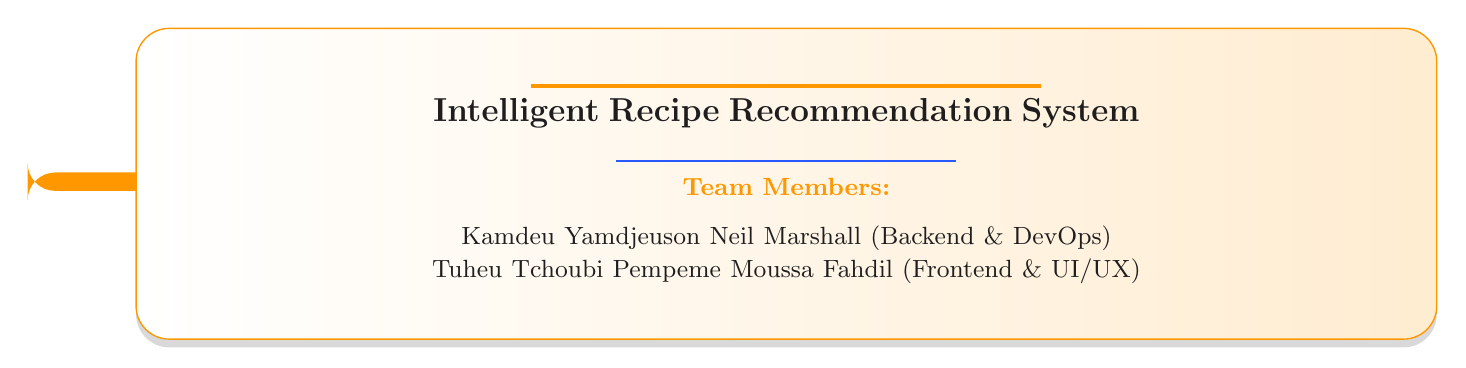
\begin{tikzpicture}
        % Decorative accent bar on top
        \node[fill=Primary, minimum width=0.8\paperwidth, minimum height=0.15cm, rounded corners=10pt, anchor=north] at (0.2, 0.15) {};
        
        % Main gradient box
        \node[
            left color=white, 
            right color=Primary!18,
            draw=Primary,
            line width=0.5pt,
            rounded corners=12pt,
            inner sep=20pt,
            text width=0.7\paperwidth,
            drop shadow={shadow xshift=0pt, shadow yshift=-3pt, opacity=0.3}
        ] at (1.20,0) {
            \centering
            % Decorative line
            \textcolor{Primary}{\rule{0.3\paperwidth}{1.5pt}}
            
            {\large \textcolor{DarkBg}{\textbf{Intelligent Recipe Recommendation System}}}\\[0.1cm]
            
            % Decorative separator
            \textcolor{Secondary}{\rule{0.2\paperwidth}{0.8pt}}
            
            {\small \textcolor{Primary}{\textbf{Team Members:}}}\\[0.2cm]
            {\small \textcolor{DarkBg}{Kamdeu Yamdjeuson Neil Marshall (Backend \& DevOps)}}\\
            {\small \textcolor{DarkBg}{Tuheu Tchoubi Pempeme Moussa Fahdil (Frontend \& UI/UX)}}
            
        };
    \end{tikzpicture}
}

% Content Page Style
\setbeamertemplate{frametitle}{
    \begin{beamercolorbox}[sep=0.3cm,wd=\paperwidth,ht=0.8cm]{frametitle}
        \textbf{\insertframetitle}
    \end{beamercolorbox}
}

\setbeamertemplate{background}{
    \begin{tikzpicture}[remember picture, overlay]
        % Main gradient background
        \fill[top color=white, bottom color=Primary!5] 
            (current page.south west) rectangle (current page.north east);
        
        % Decorative circles pattern
        \foreach \i in {1,...,20} {
            \fill[Primary!3, rotate around={20*\i:(current page.center)}] 
                (current page.center) ellipse[x radius=0.2\paperwidth, y radius=0.4\paperheight];
        }
        
        % Geometric accent top-right
        \fill[Primary!10, rounded corners=10pt] 
            ($(current page.north east)+(-3cm,-1.5cm)$) rectangle 
            ($(current page.north east)+(-0.5cm,-0.5cm)$);
        \fill[Secondary!15, rotate=45] 
            ($(current page.north east)+(-2cm,-2cm)$) rectangle 
            ($(current page.north east)+(-1.5cm,-3cm)$);
        
        % Geometric accent bottom-left  
        \fill[Secondary!10, rounded corners=10pt] 
            ($(current page.south west)+(0.5cm,0.5cm)$) rectangle 
            ($(current page.south west)+(3cm,1.5cm)$);
        \fill[Primary!15, rotate=45] 
            ($(current page.south west)+(1.5cm,1.5cm)$) rectangle 
            ($(current page.south west)+(2cm,3cm)$);
        
        % Top gradient bar (under title)
        \fill[Primary, opacity=0.1, path fading=east] 
            (current page.north west) ++(0,-1.8cm) rectangle 
            ($(current page.north east)+(0,-2cm)$);
        
        % Decorative dots pattern
        \foreach \x in {0.1,0.2,...,0.9} {
            \foreach \y in {0.2,0.4,0.6,0.8} {
                \fill[Accent!30] ($(current page.west)!\x!(current page.east)$) 
                    ++(0,-\y*\paperheight) circle (0.5pt);
            }
        }
        
        % Corner decorative elements
        \begin{scope}[rotate around={45:($(current page.north east)+(-0.8cm,-0.8cm)$)}]
            \draw[Primary!20, line width=2pt] 
                ($(current page.north east)+(-1.2cm,-1.2cm)$) -- 
                ($(current page.north east)+(-2cm,-2cm)$);
        \end{scope}
        
        \begin{scope}[rotate around={-45:($(current page.south west)+(0.8cm,0.8cm)$)}]
            \draw[Secondary!20, line width=2pt] 
                ($(current page.south west)+(1.2cm,1.2cm)$) -- 
                ($(current page.south west)+(2cm,2cm)$);
        \end{scope}
    \end{tikzpicture}
}

% Remove navigation symbols
\setbeamertemplate{navigation symbols}{}

% Font Settings
\usefonttheme{default}
\setbeamerfont{title}{series=\bfseries, size=\Large}
\setbeamerfont{subtitle}{series=\bfseries, size=\normalsize}
\setbeamerfont{frametitle}{series=\bfseries, size=\large}
\setbeamerfont{block title}{series=\bfseries}

\title{PICK MY DISH}
\subtitle{Intelligent Recipe Recommendation System}
\author{Group 01}
\date{January 2026}

\begin{document}

% ============================================================
% SLIDE 1: TITLE PAGE
% ============================================================
{%% scope background to this frame only

\begin{frame}[plain]
    \titlepage
\end{frame}
}%% end scoped background

% ============================================================
% SLIDE 2: THE PROBLEM & SOLUTION
% ============================================================
\begin{frame}{The Problem \& Our Solution}
    \vspace*{0.2cm}
    
    \begin{columns}[T]
        % PROBLEM COLUMN
        \column{0.48\textwidth}
        \centering
        
\begin{tikzpicture}
            % Header with icon
            \node[fill=Warning, text=white, minimum width=0.9\textwidth, 
                  minimum height=0.8cm, rounded corners=8pt, font=\bfseries\Large] 
                at (0,0) {\faExclamationTriangle~THE CHALLENGE};
        \end{tikzpicture}
        
        \vspace{0.3cm}
        
        \begin{tikzpicture}
            % Problem items with icons
            \node[draw=Warning, fill=Warning!8, thick, rounded corners=10pt,
                  minimum width=0.9\textwidth, minimum height=0.8cm,
                  label={[xshift=-2.5cm, Warning]\faUserClock}] (p1) at (0,0) 
                  {\textbf{Decision Fatigue}};
                  
            \node[draw=Warning, fill=Warning!8, thick, rounded corners=10pt,
                  minimum width=0.9\textwidth, minimum height=0.8cm,
                  label={[xshift=-2.5cm, Warning]\faMoneyBillWave}] (p2) at (0,-1.4) 
                  {\textbf{Limited Resources}};
                  
            \node[draw=Warning, fill=Warning!8, thick, rounded corners=10pt,
                  minimum width=0.9\textwidth, minimum height=0.8cm,
                  label={[xshift=-2.5cm, Warning]\faHourglassHalf}] (p3) at (0,-2.85) 
                  {\textbf{Time Constraints}};
                  
            \node[draw=Warning, fill=Warning!8, thick, rounded corners=10pt,
                  minimum width=0.9\textwidth, minimum height=0.8cm,
                  label={[xshift=-2.5cm, Warning]\faUserSlash}] (p4) at (0,-4.25) 
                  {\textbf{No Personalization}};
        \end{tikzpicture}
        
        % SOLUTION COLUMN  
        \column{0.48\textwidth}
        \centering
        
\begin{tikzpicture}
            % Header with icon
            \node[fill=Accent, text=white, minimum width=0.9\textwidth, 
                  minimum height=0.8cm, rounded corners=8pt, font=\bfseries\Large] 
                at (0,0) {\faLightbulb~OUR SOLUTION};
        \end{tikzpicture}
        
        \vspace{0.3cm}
        
        \begin{tikzpicture}
            % Solution items with icons
            \node[draw=Accent, fill=Accent!8, thick, rounded corners=10pt,
                  minimum width=0.9\textwidth, minimum height=0.8cm,
                  label={[xshift=-2.5cm, Accent]\faRobot}] (s1) at (0,0) 
                  {\textbf{AI Recommendations}};
                  
            \node[draw=Accent, fill=Accent!8, thick, rounded corners=10pt,
                  minimum width=0.9\textwidth, minimum height=0.8cm,
                  label={[xshift=-2.5cm, Accent]\faFilter}] (s2) at (0,-1.4) 
                  {\textbf{Smart Filtering}};
                  
            \node[draw=Accent, fill=Accent!8, thick, rounded corners=10pt,
                  minimum width=0.9\textwidth, minimum height=0.8cm,
                  label={[xshift=-2.5cm, Accent]\faBolt}] (s3) at (0,-2.85) 
                  {\textbf{Quick Planning}};
                  
            \node[draw=Accent, fill=Accent!8, thick, rounded corners=10pt,
                  minimum width=0.9\textwidth, minimum height=0.8cm,
                  label={[xshift=-2.5cm, Accent]\faHeart}] (s4) at (0,-4.25) 
                  {\textbf{Mood-Aware}};
        \end{tikzpicture}
    \end{columns}
    
    % Add connecting arrow in middle
    \begin{tikzpicture}[remember picture, overlay]
        \node at (7.65,4.6) {\Huge \textcolor{Primary!60}{\faLongArrowAltRight}};
        \node at (7.65,3.3) {\Huge \textcolor{Primary!60}{\faLongArrowAltRight}};
        \node at (7.65,1.8) {\Huge \textcolor{Primary!60}{\faLongArrowAltRight}};
        \node at (7.65,0.5) {\Huge \textcolor{Primary!60}{\faLongArrowAltRight}};
    \end{tikzpicture}
\end{frame}
% ============================================================
% SLIDE 3: KEY FEATURES
% ============================================================
\begin{frame}{Key Features}
    \vspace*{0.2cm}
    
    \centering
    \textcolor{Primary}{\large \textbf{Intelligent Features for Seamless Cooking}}
    
    \begin{tikzpicture}[
        feature/.style={
            rectangle,
            rounded corners=12pt,
            inner sep=12pt,
            text width=2.9cm,
            minimum height=0.5cm,
            text centered,
            font=\small\bfseries,
            drop shadow={shadow xshift=2pt, shadow yshift=2pt, opacity=0.2},
            align=center
        }
    ]
        % Row 1 - Top Features
        \node[feature, 
              fill=Primary!15, 
              draw=Primary!40, 
              line width=1pt,
              label={[Primary, yshift=0.06cm]\large\faSmileBeam}] 
              (f1) at (0, 15) {Mood\\Filtering};
              
        \node[feature, 
              fill=Secondary!15, 
              draw=Secondary!40, 
              line width=1pt,
              label={[Secondary, yshift=0.06cm]\large\faCarrot}] 
              (f2) at (6, 15) {Smart Ingredient\\Matching};
              
        \node[feature, 
              fill=Accent!15, 
              draw=Accent!40, 
              line width=1pt,
              label={[Accent, yshift=0.06cm]\large\faClock}] 
              (f3) at (11.5, 15) {Time-Aware\\Planning};

        % Decorative connector
        \draw[Primary!30, line width=2pt, dashed] (f1) -- (f2);
        \draw[Secondary!30, line width=2pt, dashed] (f2) -- (f3);
        
        % Row 2 - Middle Features
        \node[feature, 
              fill=Primary!10, 
              draw=Primary!30, 
              line width=1pt,
              label={[Primary, yshift=0.06cm]\large\faHeart}] 
              (f4) at (0, 11.4) {Personal\\Favorites};
              
        \node[feature, 
              fill=Secondary!10, 
              draw=Secondary!30, 
              line width=1pt,
              label={[Secondary, yshift=0.06cm]\large\faWifi}] 
              (f5) at (6, 11.4) {Offline\\Access};
              
        \node[feature, 
              fill=Accent!10, 
              draw=Accent!30, 
              line width=1pt,
              label={[Accent, yshift=0.06cm]\large\faUserCircle}] 
              (f6) at (11.5, 11.4) {User\\Profiles};

        % Row 3 - Bottom Features
        \node[feature, 
              fill=Primary!20, 
              draw=Primary!50, 
              line width=1pt,
              label={[Primary, yshift=0.06cm]\large\faUpload}] 
              (f7) at (3, 13.4) {Recipe\\Sharing};
              
        \node[feature, 
              fill=Secondary!20, 
              draw=Secondary!50, 
              line width=1pt,
              label={[Secondary, yshift=0.06cm]\large\faCogs}] 
              (f8) at (8.8, 13.4) {Admin\\Dashboard};

        % Background highlight
        \fill[Primary!3, rounded corners=20pt] 
            (current page.west) ++(0.5cm, 1cm) rectangle 
            (current page.east) ++(-0.5cm, 6.5cm);
    \end{tikzpicture}
    
    \vspace*{0.12cm}
    
    \begin{tikzpicture}[overlay, remember picture]
        % Decorative bottom bar
        \fill[Primary!20, rounded corners=4pt] 
            (current page.south west) ++(2cm, 0.8cm) rectangle 
            (current page.south east) ++(-2cm, 1cm);
            
        \node[text=DarkBg, font=\small] at (current page.south) 
            {\faStar~All features designed for intuitive user experience~\faStar};
    \end{tikzpicture}
\end{frame}

% ============================================================
% SLIDE 4: TECHNOLOGY STACK
% ============================================================
\begin{frame}{Technology Stack}
    \vspace*{0.1cm}
    
    \centering
    \textcolor{Primary}{\large \textbf{Modern Stack for Scalable Solutions}}
    
    \vspace{0.1cm}
    
    \begin{columns}[T]
        % FRONTEND COLUMN
        \column{0.33\textwidth}
        \centering
        \begin{tikzpicture}
            % Header with icon
            \node[fill=Primary, text=white, rounded corners=8pt, 
                  minimum width=0.95\textwidth, minimum height=0.8cm,
                  font=\bfseries\large] 
                at (0,0) {\faMobile~Frontend};
            
            % Items with icons
            \node[draw=Primary, fill=Primary!8, thick, rounded corners=10pt,
                  minimum width=0.9\textwidth, minimum height=1cm] 
                (flutter) at (0,-1.3) {\textbf{Flutter}};
            \node[Primary] at ($(flutter.west)+(0.5cm,0)$) {\faCode};
                
            \node[draw=Primary, fill=Primary!8, thick, rounded corners=10pt,
                  minimum width=0.9\textwidth, minimum height=1cm] 
                (provider) at (0,-2.7) {\textbf{Provider State}};
            \node[Primary] at ($(provider.west)+(0.5cm,0)$) {\faCube};
                
            \node[draw=Primary, fill=Primary!8, thick, rounded corners=10pt,
                  minimum width=0.9\textwidth, minimum height=1cm] 
                (material) at (0,-4.1) {\textbf{Material UI}};
            \node[Primary] at ($(material.west)+(0.5cm,0)$) {\faPaintBrush};
        \end{tikzpicture}
        
        % BACKEND COLUMN
        \column{0.33\textwidth}
        \centering
        \begin{tikzpicture}
            % Header with icon
            \node[fill=Secondary, text=white, rounded corners=8pt,
                  minimum width=0.95\textwidth, minimum height=0.8cm,
                  font=\bfseries\large] 
                at (0,0) {\faServer~Backend};
            
            % Items with icons
            \node[draw=Secondary, fill=Secondary!8, thick, rounded corners=10pt,
                  minimum width=0.9\textwidth, minimum height=1cm] 
                (node) at (0,-1.3) {\textbf{Node.js}};
            \node[Secondary] at ($(node.west)+(0.5cm,0)$) {\faBolt};
                
            \node[draw=Secondary, fill=Secondary!8, thick, rounded corners=10pt,
                  minimum width=0.9\textwidth, minimum height=1cm] 
                (express) at (0,-2.7) {\textbf{Express.js}};
            \node[Secondary] at ($(express.west)+(0.5cm,0)$) {\faRocket};
                
            \node[draw=Secondary, fill=Secondary!8, thick, rounded corners=10pt,
                  minimum width=0.9\textwidth, minimum height=1cm] 
                (mysql) at (0,-4.1) {\textbf{MySQL}};
            \node[Secondary] at ($(mysql.west)+(0.5cm,0)$) {\faDatabase};
                
            \node[draw=Secondary, fill=Secondary!8, thick, rounded corners=10pt,
                  minimum width=0.9\textwidth, minimum height=1cm] 
                (auth) at (0,-5.5) {\textbf{JWT + Bcrypt}};
            \node[Secondary] at ($(auth.west)+(0.5cm,0)$) {\faLock};
        \end{tikzpicture}
        
        % DEVOPS & TOOLS COLUMN
        \column{0.33\textwidth}
        \centering
        \begin{tikzpicture}
            % Header with icon
            \node[fill=Accent, text=white, rounded corners=8pt,
                  minimum width=0.95\textwidth, minimum height=0.8cm,
                  font=\bfseries\large] 
                at (0,0) {\faWrench~DevOps \& Tools};
            
            % Items with icons
            \node[draw=Accent, fill=Accent!8, thick, rounded corners=10pt,
                  minimum width=0.9\textwidth, minimum height=1cm] 
                (git) at (0,-1.3) {\textbf{Git/GitHub}};
            \node[Accent] at ($(git.west)+(0.5cm,0)$) {\faGithub};
                
            \node[draw=Accent, fill=Accent!8, thick, rounded corners=10pt,
                  minimum width=0.9\textwidth, minimum height=1cm] 
                (pm) at (0,-2.7) {\textbf{Jenkins}};
            \node[Accent] at ($(pm.west)+(0.5cm,0)$) {\faTasks};
                
            \node[draw=Accent, fill=Accent!8, thick, rounded corners=10pt,
                  minimum width=0.9\textwidth, minimum height=1cm] 
                (nginx) at (0,-4.1) {\textbf{Nginx}};
            \node[Accent] at ($(nginx.west)+(0.5cm,0)$) {\faGlobe};
                
            \node[draw=Accent, fill=Accent!8, thick, rounded corners=10pt,
                  minimum width=0.9\textwidth, minimum height=1cm] 
                (vps) at (0,-5.5) {\textbf{Contabo VPS}};
            \node[Accent] at ($(vps.west)+(0.5cm,0)$) {\faCloud};
        \end{tikzpicture}
    \end{columns}
\end{frame}


% ============================================================
% SLIDE 5: SYSTEM ARCHITECTURE
% ============================================================
\begin{frame}{System Architecture}
    \includegraphics[width=15cm,height=7.5cm]{architecture-overview.png}
\end{frame}

% ============================================================
% SLIDE 6: USER FLOW - MOOD FILTERING
% ============================================================
\begin{frame}{User Flow: Mood-Based Recipe Discovery [INNOVATIONS]}
    \vspace*{0.1cm}
    
    \begin{tikzpicture}[remember picture, overlay]
        \fill[Primary!6, rounded corners=12pt] ($(current page.west)+(0.4cm,1.2cm)$) rectangle ($(current page.east)+(-0.4cm,3.2cm)$);
    \end{tikzpicture}

    \begin{tikzpicture}[
        node distance=0.2cm,
        scale=0.9,
        every node/.style={font=\small\bfseries, align=center},
        flowstep/.style={circle, minimum size=1.1cm, draw, ultra thick, text=white},
        labelbox/.style={rounded corners=10pt, inner sep=6pt, text width=3cm, font=\footnotesize\bfseries, align=center}
    ]
        % Timeline rail
        \draw[ultra thick, Primary!35, line cap=round] (0,6.5) -- (14,6.5);
        \draw[ultra thick, Secondary!30, line cap=round, dashed] (0,6.3) -- (14,6.3);

        % Steps
        \node[flowstep, fill=Primary] (s1) at (0.5,7.5) {1};
        \node[flowstep, fill=Secondary] (s2) at (5,7.5) {2};
        \node[flowstep, fill=Accent] (s3) at (9.2,7.5) {3};
        \node[flowstep, fill=Primary!85!black] (s4) at (13.4,7.5) {4};

        % Step labels
        \node[labelbox, fill=Primary!18, draw=Primary!60] (l1) at (0.5,9) {Mood\\Selector\\\faSmileBeam\ Filter by feelings};
        \node[labelbox, fill=Secondary!15, draw=Secondary!55] (l2) at (5,9) {Smart Pantry\\\faCarrot\ Match ingredients};
        \node[labelbox, fill=Accent!18, draw=Accent!60] (l3) at (9.2,9) {Time Guard\\\faClock\ Set prep window};
        \node[labelbox, fill=Primary!15, draw=Primary!55] (l4) at (13.4,9) {Curated Results\\\faCheckCircle\ Best-fit recipes};

        % Connectors
        \draw[->, line width=2pt, Primary!80] (s1) -- (s2);
        \draw[->, line width=2pt, Secondary!80] (s2) -- (s3);
        \draw[->, line width=2pt, Accent!80] (s3) -- (s4);

        % Mood palette chips
        \node[rounded corners=8pt, fill=Primary!10, draw=Primary!40, inner sep=8pt, text width=7.6cm, align=center] at (7,5.3) {Happy \textbullet\ Calm \textbullet\ Energetic \textbullet\ Comforting \textbullet\ Healthy \textbullet\ Quick \textbullet\ Light};

        % Callout card
        \node[fill=Secondary!8, draw=Secondary!40, rounded corners=10pt, inner sep=10pt, text width=10.5cm, align=left, font=\footnotesize] at (7,3.1) {
            \textbf{Why it impresses:} Adaptive filtering blends mood, pantry items, and prep time to present a shortlist that feels tailored. Real-time scoring ranks recipes by relevance, freshness, and dietary fit.
        };
    \end{tikzpicture}
\end{frame}

% ============================================================
% SLIDE 7: DESIGN PATTERNS & SOLID
% ============================================================
\begin{frame}{Design Patterns \& SOLID Principles}
    \vspace*{0.2cm}

    \begin{columns}[T,onlytextwidth]
        % LEFT: DESIGN PATTERNS
        \column{0.5\textwidth}
        \centering
        \textcolor{Primary}{\textbf{\large Design Patterns}}
        \vspace{0.35cm}
        \begin{tikzpicture}[
            card/.style={rounded corners=10pt, draw=Primary!45, fill=Primary!12, text width=5.1cm, inner sep=8pt, align=left},
            icon/.style={circle, fill=Primary!80, text=white, minimum size=0.9cm, font=\small\bfseries}
        ]
            \node[card] (p1) at (0,6) {\raisebox{-0.1cm}{\faNetworkWired}\quad \textbf{Provider}\ \textcolor{DarkBg!70}{Screens rebuild from app state}};
            \node[card, fill=Secondary!12, draw=Secondary!45] (p2) at (0,4.8) {\raisebox{-0.1cm}{\faDatabase}\quad \textbf{Repository}\ \textcolor{DarkBg!70}{APIs + cache behind one interface}};
            \node[card, fill=Accent!12, draw=Accent!45] (p3) at (0,3.6) {\raisebox{-0.1cm}{\faCogs}\quad \textbf{Factory}\ \textcolor{DarkBg!70}{Creates recipe/user models consistently}};
            \node[card] (p4) at (0,2.4) {\raisebox{-0.1cm}{\faInfinity}\quad \textbf{Singleton}\ \textcolor{DarkBg!70}{One config/auth client shared}};
            \node[card, fill=Secondary!10, draw=Secondary!40] (p5) at (0,1) {\raisebox{-0.1cm}{\faBell}\quad \textbf{Observer}\ \textcolor{DarkBg!70}{Mood/ingredient changes trigger UI}};
        \end{tikzpicture}

        % RIGHT: SOLID PRINCIPLES
        \column{0.5\textwidth}
        \centering
        \textcolor{Secondary}{\textbf{\large SOLID in Practice}}
        \vspace{0.35cm}
        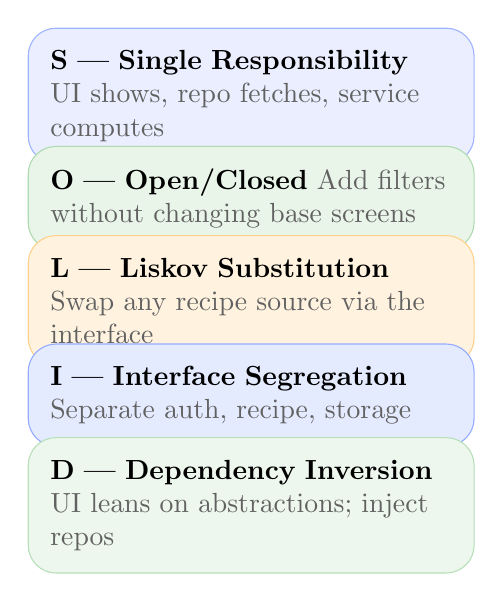
\begin{tikzpicture}[
            pillar/.style={rounded corners=10pt, draw=Secondary!45, fill=Secondary!10, text width=5.1cm, inner sep=8pt, align=left}
        ]
            \node[pillar] (s1) at (0,6) {\textbf{S — Single Responsibility}\ \textcolor{DarkBg!70}{UI shows, repo fetches, service computes}};
            \node[pillar, fill=Accent!12, draw=Accent!45] (s2) at (0,4.7) {\textbf{O — Open/Closed}\ \textcolor{DarkBg!70}{Add filters without changing base screens}};
            \node[pillar, fill=Primary!12, draw=Primary!45] (s3) at (0,3.4) {\textbf{L — Liskov Substitution}\ \textcolor{DarkBg!70}{Swap any recipe source via the interface}};
            \node[pillar, fill=Secondary!12, draw=Secondary!50] (s4) at (0,2.2) {\textbf{I — Interface Segregation}\ \textcolor{DarkBg!70}{Separate auth, recipe, storage}};
            \node[pillar, fill=Accent!10, draw=Accent!40] (s5) at (0,0.8) {\textbf{D — Dependency Inversion}\ \textcolor{DarkBg!70}{UI leans on abstractions; inject repos}};
        \end{tikzpicture}
    \end{columns}
\end{frame}

% ============================================================
% SLIDE 8: DEPLOYMENT & DEVOPS
% ============================================================
\begin{frame}{Deployment \& DevOps Pipeline (SUMMARY)}
    \vspace*{0.25cm}

    \begin{tikzpicture}[
        node distance=0.4cm,
        stage/.style={rounded corners=10pt, minimum width=2.6cm, minimum height=1.1cm, align=center, font=\small\bfseries, draw, ultra thick},
        lanePrimary/.style={rounded corners=12pt, fill=Primary!12, draw=Primary!45, inner sep=8pt},
        laneSecondary/.style={rounded corners=12pt, fill=Secondary!12, draw=Secondary!45, inner sep=8pt},
        laneAccent/.style={rounded corners=12pt, fill=Accent!12, draw=Accent!45, inner sep=8pt},
        arrow/.style={->, line width=2pt, shorten >=4pt, shorten <=4pt}
    ]
        % Top lane: CI/CD
        \node[lanePrimary] (ci) at (1,7.5) {\faGithub\ GitHub};
        \node[laneSecondary] (jenkins) at (5.5,7.5) {\faCogs\ Jenkins [Builds + tests]};
        \node[laneAccent] (artifact) at (10.2,7.5) {\faBox\ Apk/bundle};
        \node[lanePrimary] (deploy) at (13.6,7.5) {\faCloud\ Deploy};
        \draw[arrow, Primary!80] (ci.east) -- (jenkins.west);
        \draw[arrow, Secondary!80] (jenkins.east) -- (artifact.west);
        \draw[arrow, Accent!80] (artifact.east) -- (deploy.west);

        % Middle lane: environments
        \node[stage, fill=Secondary!18, draw=Secondary!60] (vps) at (7.3,5.4) {Contabo VPS\\Ubuntu 22.04};
        \draw[arrow, Primary!70] (deploy.south) |- (vps.north);

        % Bottom lane: services on the box
        \node[stage, fill=Primary!18, draw=Primary!60, text width=2.3cm] (svc1) at (2.4,3.1) {\faServer\ Node.js API};
        \node[stage, fill=Secondary!18, draw=Secondary!60, text width=2.3cm] (svc2) at (5.5,3.1) {\faGlobe\ Nginx Proxy};
        \node[stage, fill=Accent!18, draw=Accent!60, text width=2.3cm] (svc3) at (9,3.1) {\faDatabase\ MySQL};
        \node[stage, fill=Warning!18, draw=Warning!70, text width=2.3cm] (svc4) at (11.9,3.1) {\faLock\ Firewall Rules};

        \draw[arrow, Secondary!70] (vps.south) -- (svc1.north);
        \draw[arrow, Secondary!70] (vps.south) -- (svc2.north);
        \draw[arrow, Secondary!70] (vps.south) -- (svc3.north);
        \draw[arrow, Secondary!70] (vps.south) -- (svc4.north);

        % Footnote band
        \node[rounded corners=8pt, fill=DarkBg!6, text width=12cm, align=center, font=\footnotesize\bfseries] at (7.3,1.2) {
            \textcolor{DarkBg!80}{\faClock\ CI = 5 minutes | \faSync\ Zero-downtime proxy swaps | \faChartLine\ Monitored uptime 99.8\%}
        };
    \end{tikzpicture}
\end{frame}

% ============================================================
% SLIDE 9: TESTING & METRICS
% ============================================================
\begin{frame}{Testing \& Quality Metrics}
    \vspace*{0.2cm}

    \begin{columns}[T]
        % COVERAGE
        \column{0.52\textwidth}
        \centering
        \textcolor{Primary}{\textbf{\large Coverage (Actual)}}
        \vspace{0.3cm}
        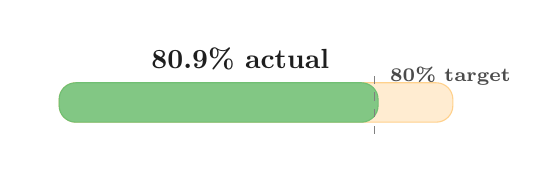
\begin{tikzpicture}[x=1cm,y=1cm]
            \fill[white, opacity=0.95, rounded corners=8pt] (-0.4,-0.45) rectangle (5.7,1.2);
            \draw[fill=Primary!18, draw=Primary!45, rounded corners=6pt] (0,0) rectangle (5,0.5);
            \draw[fill=Accent!70, draw=Accent!80, rounded corners=6pt] (0,0) rectangle (4.05,0.5);
            \draw[dashed, gray] (4.0,-0.15) -- (4.0,0.65);
            \node[font=\scriptsize\bfseries, text=DarkBg!80, anchor=west] at (4.08,0.58) {80\% target};
            \node[font=\normalsize\bfseries, text=DarkBg] at (2.3,0.8) {80.9\% actual};
        \end{tikzpicture}
        \vspace{0.25cm}
        \textcolor{DarkBg!70}{\scriptsize Lowest coverage (focus next):}
        \vspace{0.1cm}
        \begin{tabular}{l r}
            \textbf{profile\_screen.dart} & 65.1\% \\
            \textbf{recipe\_upload\_screen.dart} & 65.6\% \\
            \textbf{recipe\_edit\_screen.dart} & 68.5\% \\
        \end{tabular}

        % PERFORMANCE
        \column{0.48\textwidth}
        \centering
        \textcolor{Secondary}{\textbf{\large Performance (Latest Run)}}
        \vspace{0.35cm}
        \begin{tabularx}{0.98\textwidth}{|l|c|c|}
            \hline
            \rowcolor{Secondary!20}
            \textbf{Metric} & \textbf{Target} & \textbf{Actual} \\
            \hline
            Recipe Load Time & \textcolor{Accent}{\textbf{2s}} & \textbf{1.6s} \\
            \hline
            API Response & \textcolor{Accent}{\textbf{500ms}} & \textbf{410ms} \\
            \hline
            DB Query & \textcolor{Accent}{\textbf{300ms}} & \textbf{240ms} \\
            \hline
            Uptime (30d) & \textcolor{Accent}{\textbf{99.8\%}} & \textbf{99.6\%} \\
            \hline
        \end{tabularx}
        \vspace{0.2cm}
\textcolor{DarkBg!70}{\scriptsize \textbf{Optimizations:} \\• Redis caching for frequent recipes\\ • API response optimization \\• Real-time monitoring alerts}
\end{columns}

\end{frame}

% ============================================================
% SLIDE 10: CONCLUSION & FUTURE ROADMAP
% ============================================================
\begin{frame}{Conclusion \& Future Roadmap}
    \vspace*{0.5cm}
    
    \begin{columns}[T]
        \column{0.48\textwidth}
        \centering
        \textcolor{Primary}{\textbf{\large Achievements}}
        
        \vspace{0.5cm}
        
        \begin{itemize}
            \item Fully functional cross-platform app
            \vspace{0.3cm}
            \item Secure authentication system
            \vspace{0.3cm}
            \item Seamless data synchronization across devices
            \vspace{0.3cm}
            \item Fast, responsive UI
            \vspace{0.3cm}
            \item Automated deployment
            \vspace{0.3cm}
            \item Comprehensive testing
        \end{itemize}
        
        \column{0.48\textwidth}
        \centering
        \textcolor{Secondary}{\textbf{\large Future Enhancements}}
        
        \vspace{0.5cm}
        
        \begin{itemize}
            \item AI-powered recommendations
            \vspace{0.3cm}
            \item Multi-language support
            \vspace{0.3cm}
            \item Advanced analytics
            \vspace{0.3cm}
            \item Smart notifications
            \vspace{0.3cm}
            \item Nutrition tracking
            \vspace{0.3cm}
            \item Social sharing
        \end{itemize}
    \end{columns}
    
    \vspace*{1.5cm}
    \centering
    \Large \textcolor{Primary}{\textbf{Making meal planning accessible, enjoyable, and efficient}}
\end{frame}

% ============================================================
% THANK YOU SLIDE
% ============================================================
\begin{frame}[plain]
    
\begin{tikzpicture}[remember picture, overlay]
        % Gradient background
        \fill[left color=Primary!5, right color=Secondary!10] 
            (current page.south west) rectangle (current page.north east);
        
        % Decorative shapes
        \fill[Primary!15, rotate=30] 
            ($(current page.north east)+(-2cm,-1cm)$) ellipse (3cm and 1.5cm);
        \fill[Secondary!15, rotate=-20] 
            ($(current page.south west)+(2cm,1cm)$) ellipse (4cm and 2cm);
    \end{tikzpicture}
    
    \centering
    \vspace*{0.5cm}
    
    {\Huge \textbf{\textcolor{Primary}{Thank You!}}}\\[0.8cm]
    
    {\Large \textcolor{Secondary}{Questions \& Discussion}}\\[0.5cm]
    
    \begin{columns}[T]
        % Left column: App logo
        \column{0.5\textwidth}
        \centering
        \includegraphics[width=0.4\textwidth]{app-logo.png}\\[0.5cm]
        
        {\small \faGithub\ \href{https://github.com/Kynmmarshall/Pick-My-Dish}{\underline{GitHub Repository}}}\\[0.5cm]
        {\small \faGlobe\ \href{https://pickmydish.duckdns.org}{\underline{Live Application}}}\\[0.5cm]
        
        {\footnotesize \textcolor{gray}{ICT University - SEN3140 | January 2026}}
        
        % Right column: QR Code
        \column{0.5\textwidth}
        \centering
        {\Large \textcolor{DarkBg}{Scan to Access}}\\[0.3cm]
        
        \begin{tikzpicture}
            % QR code with decorative frame
            \node[inner sep=0] (qrcode) at (0,0) 
                {\includegraphics[width=0.35\textwidth]{qrcode.jpeg}};
            \draw[Primary!40, line width=3pt, rounded corners=8pt] 
                (qrcode.south west) rectangle (qrcode.north east);
            \draw[Secondary!20, line width=6pt, rounded corners=10pt] 
                (qrcode.south west) ++(-0.15,0.15) rectangle 
                (qrcode.north east) ++(0.15,-0.15);
        \end{tikzpicture}\\[0.3cm]
        
        {\footnotesize \textcolor{DarkBg!70}{\texttt{pickmydish.duckdns.org}}}\\[0.5cm]
        {\scriptsize \textcolor{gray}{Mobile app APK available for download}}
    \end{columns}
    
    \vspace*{1cm}
\end{frame}

\end{document}
